%%%%%%%%%%%%%%%%%%%%%%%%%%%%%%%%%%%%%%%%%%%%%%%%%%%%%%%%%%%%%%%%%%%%%%
%%  Copyright by Wenliang Du.                                       %%
%%  This work is licensed under the Creative Commons                %%
%%  Attribution-NonCommercial-ShareAlike 4.0 International License. %%
%%  To view a copy of this license, visit                           %%
%%  http://creativecommons.org/licenses/by-nc-sa/4.0/.              %%
%%%%%%%%%%%%%%%%%%%%%%%%%%%%%%%%%%%%%%%%%%%%%%%%%%%%%%%%%%%%%%%%%%%%%%

\newcommand{\commonfolder}{../../common-files}
\newcommand{\webcommon}{../Web_Common}

\documentclass[11pt]{article}

\usepackage[most]{tcolorbox}
\usepackage{times}
\usepackage{epsf}
\usepackage{epsfig}
\usepackage{amsmath, alltt, amssymb, xspace}
\usepackage{wrapfig}
\usepackage{fancyhdr}
\usepackage{url}
\usepackage{verbatim}
\usepackage{fancyvrb}
\usepackage{adjustbox}
\usepackage{listings}
\usepackage{color}
\usepackage{subfigure}
\usepackage{cite}
\usepackage{sidecap}
\usepackage{pifont}
\usepackage{mdframed}
\usepackage{textcomp}
\usepackage{enumitem}


% Horizontal alignment
\topmargin      -0.50in  % distance to headers
\oddsidemargin  0.0in
\evensidemargin 0.0in
\textwidth      6.5in
\textheight     8.9in 

\newcommand{\todo}[1]{
\vspace{0.1in}
\fbox{\parbox{6in}{TODO: #1}}
\vspace{0.1in}
}


\newcommand{\unix}{{\tt Unix}\xspace}
\newcommand{\linux}{{\tt Linux}\xspace}
\newcommand{\minix}{{\tt Minix}\xspace}
\newcommand{\ubuntu}{{\tt Ubuntu}\xspace}
\newcommand{\setuid}{{\tt Set-UID}\xspace}
\newcommand{\openssl} {\texttt{openssl}}


\pagestyle{fancy}
\lhead{\bfseries SEED Labs}
\chead{}
\rhead{\small \thepage}
\lfoot{}
\cfoot{}
\rfoot{}


\definecolor{dkgreen}{rgb}{0,0.6,0}
\definecolor{gray}{rgb}{0.5,0.5,0.5}
\definecolor{mauve}{rgb}{0.58,0,0.82}
\definecolor{lightgray}{gray}{0.90}


\lstset{%
  frame=none,
  language=,
  backgroundcolor=\color{lightgray},
  aboveskip=3mm,
  belowskip=3mm,
  showstringspaces=false,
%  columns=flexible,
  basicstyle={\small\ttfamily},
  numbers=none,
  numberstyle=\tiny\color{gray},
  keywordstyle=\color{blue},
  commentstyle=\color{dkgreen},
  stringstyle=\color{mauve},
  breaklines=true,
  breakatwhitespace=true,
  tabsize=3,
  columns=fullflexible,
  keepspaces=true,
  escapeinside={(*@}{@*)}
}

\newcommand{\newnote}[1]{
\vspace{0.1in}
\noindent
\fbox{\parbox{1.0\textwidth}{\textbf{Note:} #1}}
%\vspace{0.1in}
}


%% Submission
\newcommand{\seedsubmission}{You need to submit a detailed lab report, with screenshots,
to describe what you have done and what you have observed.
You also need to provide explanation
to the observations that are interesting or surprising.
Please also list the important code snippets followed by
explanation. Simply attaching code without any explanation will not
receive credits.}

%% Book
\newcommand{\seedbook}{\textit{Computer \& Internet Security: A Hands-on Approach}, 2nd
Edition, by Wenliang Du. See details at \url{https://www.handsonsecurity.net}.}

%% Videos
\newcommand{\seedisvideo}{\textit{Internet Security: A Hands-on Approach},
by Wenliang Du. See details at \url{https://www.handsonsecurity.net/video.html}.}

\newcommand{\seedcsvideo}{\textit{Computer Security: A Hands-on Approach},
by Wenliang Du. See details at \url{https://www.handsonsecurity.net/video.html}.}

%% Lab Environment
\newcommand{\seedenvironment}{This lab has been tested on our pre-built
Ubuntu 16.04 VM, which can be downloaded from the SEED website. }

\newcommand{\seedenvironmentA}{This lab has been tested on our pre-built
Ubuntu 16.04 VM, which can be downloaded from the SEED website. }

\newcommand{\seedenvironmentB}{This lab has been tested on our pre-built
Ubuntu 20.04 VM, which can be downloaded from the SEED website. }

\newcommand{\seedenvironmentAB}{This lab has been tested on our pre-built
Ubuntu 16.04 and 20.04 VMs, which can be downloaded from the SEED website. }

\newcommand{\nodependency}{Since we use containers to set up the lab environment, 
this lab does not depend too much on our SEED VM. You can do this lab
using other VMs or physical machines. }







\newcommand{\seedlabcopyright}[1]{
\vspace{0.1in}
\fbox{\parbox{6in}{\small Copyright \copyright\ {#1}\ \ by Wenliang Du.\\
      This work is licensed under a Creative Commons
      Attribution-NonCommercial-ShareAlike 4.0 International License.
      If you remix, transform, or build upon the material, 
      this copyright notice must be left intact, or reproduced in a way that is reasonable to
      the medium in which the work is being re-published.}}
\vspace{0.1in}
}






\lhead{\bfseries SEED Labs -- CSRF Lab}

\begin{document}

\begin{center}
{\LARGE Cross-Site Request Forgery (CSRF) Attack Lab}
\vspace{0.1in}\\
{\Large (Web Application: {\tt Elgg})}
\end{center}

\seedlabcopyright{2006 - 2020}



% *******************************************
% SECTION
% ******************************************* 
\section{Overview}


The objective of this lab is to help students understand the Cross-Site Request
Forgery (CSRF) attack. A CSRF attack involves a victim user, a
trusted site, and a malicious site. The victim user holds an active session
with a trusted site while visiting a malicious site. The
malicious site injects an HTTP request for the trusted site into the victim
user session, causing damages.

In this lab, students  will be attacking a social networking web
application using the CSRF attack. The open-source social networking application is called 
\texttt{Elgg}, which has already been installed in our VM.
\texttt{Elgg} has countermeasures against CSRF, but we have turned them off for the
purpose of this lab.  This lab covers the following topics:

\begin{itemize}[noitemsep]
 \item Cross-Site Request Forgery attack
 \item CSRF countermeasures: Secret token and Same-site cookie
 \item HTTP GET and POST requests
 \item JavaScript and Ajax
\end{itemize}


\paragraph{Readings.}
Detailed coverage of the CSRF attack can be found in the following:

\begin{itemize}
\item Chapter 10 of the SEED Book, \seedbook
\end{itemize}


\paragraph{Lab environment.} \seedenvironmentB \nodependency



% *******************************************
% SECTION
% *******************************************
\section{Lab Environment Setup}

In this lab, we will use two websites. 
The first website is the vulnerable Elgg
site accessible at \url{www.csrflabelgg.com}. The second
website is the attacker's malicious web site that is used for
attacking Elgg. This web site is accessible via
\url{www.csrflab-attacker.com}. We use containers to
set up the lab environment.


% -------------------------------------------
% SUBSECTION
% -------------------------------------------
\subsection{Container Setup and Commands}

%%%%%%%%%%%%%%%%%%%%%%%%%%%%%%%%%%%%%%%%%%%%
Please download the
\texttt{Labsetup.zip} file to your VM from the lab's website,
unzip it, enter the \texttt{Labsetup} folder, and 
use the \texttt{docker-compose.yml} file to 
set up the lab environment. Detailed explanation
of the content in this file and all the involved 
\texttt{Dockerfile} can be found from the 
user manual, which is linked to the website of this lab.
If this is the first time you set up a SEED lab environment
using containers, it is very important that you read 
the user manual. 

In the following, we list some of the commonly
used commands related to Docker and Compose. 
Since we are going to use 
these commands very frequently, we have created aliases for them
in the \texttt{.bashrc} file (in our provided SEEDUbuntu 20.04 VM).


\begin{lstlisting}
$ docker-compose build  # Build the container image
$ docker-compose up     # Start the container
$ docker-compose down   # Shut down the container

// Aliases for the Compose commands above
$ dcbuild       # Alias for: docker-compose build
$ dcup          # Alias for: docker-compose up
$ dcdown        # Alias for: docker-compose down
\end{lstlisting}


All the containers will be running in the background. To run
commands on a container, we often need to get a shell on
that container. We first need to use the \texttt{"docker ps"}  
command to find out the ID of the container, and then
use \texttt{"docker exec"} to start a shell on that 
container. We have created aliases for them in
the \texttt{.bashrc} file.

\begin{lstlisting}
$ dockps        # Alias for: docker ps --format "{{.ID}}  {{.Names}}" 
$ docksh <id>   # Alias for: docker exec -it <id> /bin/bash

# The following example shows how to get a shell inside hostC
$ dockps
b1004832e275  hostA-10.9.0.5
0af4ea7a3e2e  hostB-10.9.0.6
9652715c8e0a  hostC-10.9.0.7

$ docksh 96
root@9652715c8e0a:/#  

# Note: If a docker command requires a container ID, you do not need to 
#       type the entire ID string. Typing the first few characters will 
#       be sufficient, as long as they are unique among all the containers. 
\end{lstlisting}


If you encounter problems when setting up the lab environment, 
please read the ``Common Problems'' section of the manual
for potential solutions.


%%%%%%%%%%%%%%%%%%%%%%%%%%%%%%%%%%%%%%%%%%%%


% -------------------------------------------
% SUBSECTION
% -------------------------------------------
\subsection{Elgg Web Application}

We use an open-source web application called Elgg in this lab.
Elgg is a web-based social-networking application.
It is already set up in the provided container images.
We use two containers, one running the web server (\texttt{10.9.0.5}) ,
and the other running the MySQL database (\texttt{10.9.0.6}).
The IP addresses for these two containers are hardcoded in various
places in the configuration, so please do not change them from
the \texttt{docker-compose.yml} file.

\paragraph{The Elgg container.}
We host the Elgg web application using the Apache web server.
The website setup is included in
\texttt{apache\_elgg\_csrf.conf} inside the Elgg image folder.
The configuration specifies the URL for the website and
the folder where the web application code is stored.

\begin{lstlisting}
<VirtualHost *:80>
     DocumentRoot /var/www/elgg
     ServerName www.csrflabelgg.com
     <Directory /var/www/elgg>
          Options FollowSymlinks
          AllowOverride All
          Require all granted
     </Directory>
</VirtualHost>
\end{lstlisting}

\paragraph{The Attacker container.}
We use another container (\texttt{10.9.0.105}) for the 
attacker machine, which hosts a malicious website. 
The Apache configuration for this website is listed
in the following:

\begin{lstlisting}
<VirtualHost *:80>
    ServerName www.csrflab-attacker.com
    DocumentRoot /var/www/attacker
</VirtualHost>
\end{lstlisting}
 
Since we need to create web pages inside this container,
for convenience, as well as for keeping the pages we have created, 
we mounted a folder (\texttt{Labsetup/attacker} on the 
hosting VM) to the container's \texttt{/var/www/attacker}
folder, which is the \texttt{DocumentRoot} folder in our Apache
configuration. Therefore, the web pages we 
put inside the \texttt{attacker} folder on the VM
will be hosted by the attacker's website. 
We have already placed some code skeletons inside 
this folder. 


\paragraph{DNS configuration.}
We access the Elgg website and attacker 
websites on the VM using their respective URLs. 
The URLs are only accessible from inside of the virtual machine, because we
have modified the \texttt{/etc/hosts} file to map the hostname
of the URLs to the IP address of their containers:

\begin{lstlisting}
10.9.0.5    www.csrflabelgg.com
10.9.0.105  www.csrflab-attacker.com
\end{lstlisting}


\vspace{-0.1in}
% MySQL database
%%%%%%%%%%%%%%%%%%%%%%%%%%%%%%%%%%%%

\paragraph{MySQL database.}
Containers are usually disposable, so once it
is destroyed, all the data inside the containers are lost.
For this lab, we do want to keep the data in the
MySQL database, so we do not lose our work when we shutdown
our container. To achieve this,
we have mounted the \texttt{mysql\_data} folder on
the host machine (inside
\texttt{Labsetup}, it will be created after the
MySQL container runs once) to the
\texttt{/var/lib/mysql} folder
inside the MySQL container.
This folder is where
MySQL stores its database. Therefore,
even if the container is destroyed,
data in the database are still kept.
If you do want to start from a clean
database, you can remove this folder:

\begin{lstlisting}
$ sudo rm -rf mysql_data
\end{lstlisting}


%%%%%%%%%%%%%%%%%%%%%%%%%%%%%%%%%%%%


\vspace{-0.1in}
%%%%%%%%%%%%%%%%%%%%%%%%%%%%%%%%%%%%
%%%%%%%%%%%%%%%%%%%%%%%%%%%%%%%%%%%%%%%%%%%%%%%%%%%%%%%%%%%%%%%%%%%%%%
%%  Copyright by Wenliang Du.                                       %%
%%  This work is licensed under the Creative Commons                %%
%%  Attribution-NonCommercial-ShareAlike 4.0 International License. %%
%%  To view a copy of this license, visit                           %%
%%  http://creativecommons.org/licenses/by-nc-sa/4.0/.              %%
%%%%%%%%%%%%%%%%%%%%%%%%%%%%%%%%%%%%%%%%%%%%%%%%%%%%%%%%%%%%%%%%%%%%%%


\paragraph{User accounts.}
We have created several user accounts on the {\tt Elgg} server; 
the user name and passwords are given in the following.


\begin{lstlisting}
----------------------------
UserName  | Password
----------------------------
admin     |  seedelgg
alice     |  seedalice 
boby      |  seedboby 
charlie   |  seedcharlie 
samy      |  seedsamy 
----------------------------
\end{lstlisting}





%%%%%%%%%%%%%%%%%%%%%%%%%%%%%%%%%%%%


% *******************************************
% SECTION
% ******************************************* 
\section{Lab Tasks: Attacks}


% -------------------------------------------
% SUBSECTION
% ------------------------------------------- 
\subsection{Task 1: Observing HTTP Request.}

In Cross-Site Request Forget attacks, we need to forge HTTP requests. 
Therefore, we need to know what a legitimate HTTP request looks like and 
what parameters it uses, etc. 
We can use a Firefox add-on called \texttt{"HTTP Header Live"} for this
purpose.  
The goal of this task is to get familiar with this tool. 
Instructions on how to use this tool is given in the Guideline
section~(\S~\ref{web:sec:httpheaderlive}).
Please use this tool to capture an HTTP GET request and an HTTP POST
request in Elgg. In your report, please identify the parameters
used in this these requests, if any. 



% -------------------------------------------
% SUBSECTION
% ------------------------------------------- 
\subsection{Task 2: CSRF Attack using GET Request}

In this task, we need two people in the Elgg social network: Alice
and Samy. Samy wants to become a friend to Alice, but Alice refuses to add 
him to her Elgg friend list. Samy decides to use the CSRF attack to
achieve his goal. He sends Alice an URL (via an email or a posting in 
Elgg); Alice, curious about it, clicks on the URL, which leads her to Samy's web site:    
{\tt www.csrflab-attacker.com}. Pretend that you are Samy, describe how you
can construct the content of the web page, so as soon as Alice visits the
web page, Samy is added to the friend list of Alice (assuming Alice has an
active session with Elgg).


To add a friend to the victim, we need to identify what the legitimate 
Add-Friend HTTP request (a GET request) looks like. We can use 
the \texttt{"HTTP Header Live"} Tool to do the investigation. 
In this task, you are not allowed to
write JavaScript code to launch the CSRF attack. Your job is to make the
attack successful as soon as Alice visits the web page, without even making
any click on the page (hint: you can use the {\tt img} tag, which
automatically triggers an HTTP GET request).
 

Elgg has implemented a countermeasure to defend against 
CSRF attacks. In Add-Friend HTTP requests, you may notice that each 
request includes two wired-looking parameters, \texttt{\_\_elgg\_ts} and 
\texttt{\_\_elgg\_token}. These parameters are used by the countermeasure, so if they do not
contain correct values, the request will not be accepted by Elgg.   
We have disabled the countermeasure for this lab, so there is no need to include these two 
parameters in the forged requests. 


% -------------------------------------------
% SUBSECTION
% ------------------------------------------- 
\subsection{Task 3: CSRF Attack using POST Request}

After adding himself to Alice's friend list, Samy wants to do something more. He 
wants Alice to say ``Samy is my Hero'' in her profile, so everybody knows 
about that. Alice does not like Samy, let alone putting that statement 
in her profile. Samy plans to use a CSRF attack to achieve that goal. 
That is the purpose of this task. 


One way to do the attack is to post a message to Alice's Elgg account, hoping that 
Alice will click the URL inside the message. This URL will lead Alice to your (i.e., Samy's)
malicious web site \url{www.csrflab-attacker.com}, where you can launch the
CSRF attack. 

The objective of your attack is to modify the victim's profile. 
In particular, the attacker needs to forge a request 
to modify the profile information of the victim user of Elgg. 
Allowing users to modify their profiles is a feature of 
Elgg. If  users want to modify their profiles,
they go to the profile page of Elgg, fill out 
a form, and then submit the form---sending a POST request---to 
the server-side script {\tt /profile/edit.php}, which 
processes the request and does the profile modification.


The server-side script {\tt edit.php} accepts both GET and POST requests,
so you can use the same trick as that in Task 1 to achieve the attack.
However, in this task, you are required to use the POST request. 
Namely, attackers (you) need to forge an HTTP POST request from the victim's
browser, when the victim is visiting their malicious site. 
Attackers need to know the structure of such a request.
You can observe the
structure of the request, i.e.,  the parameters of the request, by making
some modifications to the profile and monitoring the request using
the \texttt{"HTTP Header Live"} tool. 
You may see something similar to
the following. Unlike HTTP {\tt GET} requests, which append 
parameters to the URL strings, the parameters of HTTP {\tt POST} requests are 
included in the HTTP message body (see the contents between the two 
\ding{80} symbols): 


\begin{lstlisting}
http://www.csrflabelgg.com/action/profile/edit

POST /action/profile/edit HTTP/1.1
Host: www.csrflabelgg.com
User-Agent: Mozilla/5.0 (X11; Ubuntu; Linux i686; rv:23.0) ...
Accept: text/html,application/xhtml+xml,application/xml;q=0.9,*/*;q=0.8
Accept-Language: en-US,en;q=0.5
Accept-Encoding: gzip, deflate
Referer: http://www.csrflabelgg.com/profile/elgguser1/edit
Cookie: Elgg=p0dci8baqrl4i2ipv2mio3po05
Connection: keep-alive
Content-Type: application/x-www-form-urlencoded
Content-Length: 642
__elgg_token=fc98784a9fbd02b68682bbb0e75b428b&__elgg_ts=1403464813  (*@\ding{80}@*) 
&name=elgguser1&description=%3Cp%3Iamelgguser1%3C%2Fp%3E
&accesslevel%5Bdescription%5D=2&briefdescription= Iamelgguser1
&accesslevel%5Bbriefdescription%5D=2&location=US
......                                                              (*@\ding{80}@*)
\end{lstlisting}


After understanding the structure of the request, you need to 
be able to generate the request from your attacking web page
using JavaScript code. 
To help you write such a JavaScript program,  we provide a 
sample code in the following You can use this sample code to construct your malicious web site
for the CSRF attacks. This is only a sample code, and you need to modify it to 
make it work for your attack.


\begin{lstlisting}
<html>
<body>
<h1>This page forges an HTTP POST request.</h1>
<script type="text/javascript">

function forge_post()
{
    var fields;

    // The following are form entries need to be filled out by attackers. 
    // The entries are made hidden, so the victim won't be able to see them.
    fields += "<input type='hidden' name='name' value='****'>";
    fields += "<input type='hidden' name='briefdescription' value='****'>";
    fields += "<input type='hidden' name='accesslevel[briefdescription]' 
                                    value='2'>";                         (*@\ding{192}@*)
    fields += "<input type='hidden' name='guid' value='****'>";

    // Create a <form> element.
    var p = document.createElement("form");
	 
    // Construct the form
    p.action = "http://www.example.com";
    p.innerHTML = fields;
    p.method = "post";
	 
    // Append the form to the current page.
    document.body.appendChild(p);
	 
    // Submit the form
    p.submit();
}

	
// Invoke forge_post() after the page is loaded.
window.onload = function() { forge_post();}
</script>
</body>
</html>
\end{lstlisting}


In Line~\ding{192}, the value \texttt{2} sets the access level of a field to public. 
This is needed, otherwise, the access level will be set by default to private, so others cannot
see this field. It should be noted that when copy-and-pasting the above code
from a PDF file, the  single quote character in the program may become 
something else (but still looks like a single quote). That will cause 
syntax errors. Replace all the single quote symbols with the one typed from 
your keyboard will fix those errors. 


\paragraph{Questions.}
In addition to describing your attack in full details, you also need to
answer the following questions in your report:

\begin{itemize}
   \item \textbf{Question 1}: The forged HTTP request needs Alice's user
   id (guid) to work properly. If Boby targets Alice specifically, before
   the attack, he can find ways to get Alice's user id. Boby does not know 
   Alice's Elgg password, so he cannot log into Alice's account to get
   the information. Please describe how Boby can solve this problem.

   
   \item \textbf{Question 2:} If Boby would like to launch the attack to
   anybody who visits his malicious web page. In this case, he does not
   know who is visiting the web page beforehand. Can he still launch the CSRF attack
   to modify the victim's Elgg profile? Please explain.
\end{itemize}





% *******************************************
% SECTION
% *******************************************
\section{Lab Tasks: Defense} 

CSRF is not difficult to defend against. Initially, most applications
put a secret token in their pages, and by checking whether the token
is present in the request or not, they can tell whether a request
is a same-site request or a cross-site request. This is called
\textit{secret token} approach. 
More recently,
most browsers have implemented a mechanism called 
\textit{SameSite cookie}, which is intended to simplify the 
implementation of CSRF countermeasures. We will 
conduct experiments on both methods. 


% -------------------------------------------
% SUBSECTION
% ------------------------------------------- 
\subsection{Task 4: Enabling Elgg's Countermeasure} 

To defend against CSRF attacks, web applications can embed a secret token
in their pages. All the requests coming from these pages must carry this 
token, or they will be considered as a cross-site request, and will
not have the same privilege as the same-site requests. 
Attacker will not be able to get this secret token, so their requests
are easily identified as cross-site requests. 


Elgg uses this secret-token approach as its 
built-in countermeasures to defend against CSRF attacks. 
We have disabled the countermeasures to make the attack work. 
Elgg embeds two parameters
{\tt\_\_elgg\_ts} and {\tt\_\_elgg\_token} in the request.
The two parameters are added to the HTTP message body for the POST requests and to the URL
string for the HTTP GET requests. The server will validate them
before processing a request. 


\paragraph{Embedding secret token and timestamp to web pages.}
Elgg adds security token and timestamp to all the HTTP requests. 
The following HTML code is present in all the forms where user action is required. 
These are two hidden fields; when the form is submitted, these
two hidden parameters are added to the request:

\begin{lstlisting}
<input type = "hidden" name = "__elgg_ts" value = "" />
<input type = "hidden" name = "__elgg_token" value = "" />
\end{lstlisting}

Elgg also assign the values of the security token and timestamp to JavaScript variables, 
so they can be easily accessed by the JavaScript code on the same page.

\begin{lstlisting}
elgg.security.token.__elgg_ts;
elgg.security.token.__elgg_token;
\end{lstlisting}


The secret token and timestamp are added to Elgg's web pages by the 
\path{vendor/elgg/elgg/views/default/input/securitytoken.php} 
module. The code snippet below shows how they are dynamically 
added to web pages.

\begin{lstlisting}
$ts = time();
$token = elgg()->csrf->generateActionToken($ts);

echo elgg_view('input/hidden', ['name' => '__elgg_token', 'value' => $token]);
echo elgg_view('input/hidden', ['name' => '__elgg_ts', 'value' => $ts]);
\end{lstlisting}


\paragraph{Secret token generation.}
Elgg's security token is a hash value (md5 message digest) of the site 
secret value (retrieved from database),
timestamp, user session ID and random generated session string. 
The code below shows the secret token generation in Elgg 
(in \path{vendor/elgg/elgg/engine/classes/Elgg/Security/Csrf.php}).

\begin{lstlisting}
/**
 * Generate a token from a session token (specifying the user), 
 * the timestamp, and the site key.
 */
public function generateActionToken($timestamp, $session_token = '') {
  if (!$session_token) {
          $session_token = $this->session->get('__elgg_session');
          if (!$session_token) {
                  return false;
          }
  }

  return $this->hmac
          ->getHmac([(int) $timestamp, $session_token], 'md5')
          ->getToken();
}
\end{lstlisting}


\paragraph{Secret token validation.}
The elgg web application validates the generated token and timestamp to
defend against the CSRF attack.  Every user action calls the 
\texttt{validate} function inside \texttt{Csrf.php}, and this function validates the tokens.
If tokens are not present or invalid, the action will be denied and the
user will be redirected. In our setup, we added 
a \texttt{return} at the beginning of this function, essentially
disabling the validation.

\begin{lstlisting}
public function validate(Request $request) {
   (*@\textbf{return;}@*) // Added for SEED Labs (disabling the CSRF countermeasure)

   $token = $request->getParam('__elgg_token');
   $ts = $request->getParam('__elgg_ts');
   ... (code omitted) ...
}
\end{lstlisting}



\paragraph{Task: Turn on countermeasure.}
To turn on the countermeasure, just remove the \texttt{return}
from the \texttt{Csrf.php} file inside the \texttt{image\_elgg/elgg} 
folder (on your host VM), rebuild the container images, and restart all 
the containers. Then repeat the attack again, and see whether your attack will
be successful or not. 
Please point out the secret tokens in the captured HTTP requests.
Please explain why
the attacker cannot send these secret tokens in the CSRF attack; what
prevents them from finding out the secret tokens from the web page?   





% -------------------------------------------
% SUBSECTION
% -------------------------------------------
\subsection{Task 5: Experimenting with the SameSite Cookie Method} 

Most browsers have now implemented a mechanism called SameSite cookie, 
which is a property associated with cookies. When sending out 
requests, browsers will check this property, and decide whether 
to attach the cookie in a cross-site request. A web application can
set a cookie as SameSite if it does not want the cookie to be 
attached to cross-site requests. For example, they can mark
the session ID cookie as SameSite, so no cross-site request
can use the session ID, and will therefore not be able to 
launch CSRF attacks. 


To help students get an idea on how the SameSite cookies can
help defend against CSTF attacks, we have created a website
called \url{www.csrflab-defense.com} on one of the containers. Please 
visit the following URL (the hostname is already mapped 
to \texttt{10.9.0.5} in the \texttt{/etc/hosts} file; if you are 
not using the SEED VM, you should add this mapping to your machine): 

\begin{lstlisting}
URL: http://www.csrflab-defense.com/
\end{lstlisting}

Once you have visited this website once, three cookies will be 
set on your browser, \texttt{cookie-normal}, \texttt{cookie-lax},
and \texttt{cookie-strict}. As indicated by the name,
the first cookie is just a normal one, the second and third cookies
are samesite cookies of two different types (\texttt{Lax} and \texttt{Strict}
types). We have designed two sets of experiments to see 
which cookies will be attached when you send an HTTP request
back to the server. Typically, all the cookies belonging to the server
will be attached, but this is not the case if a cookie is a samesite type. 


Please follow the links for the two experiments. Link A points to a page 
on \url{csrflab-defense.com}, while Link B points to a page 
on \url{csrflab-attacker.com}. Both pages are identical (except for the background
color), and they both send three different types of requests to
\url{www.csrflab-defense.com/showcookies.php}, which
simply displays the cookies sent by the browser. By looking 
at the display results, you can tell which cookies were sent 
by the browser. Please do the following: 


\begin{itemize}
\item Please describe what you see and explain why some cookies are 
not sent in certain scenarios. 
 
\item Based on your understanding, please describe how the SameSite
cookies can help a server detect whether a request 
is a cross-site or same-site request. 

\item Please describe how you would use
the SameSite cookie mechanism to help Elgg defend against CSRF attacks. 
You only need to describe general ideas, and there is no need to 
implement them. 
\end{itemize}


\paragraph{Bonus points.} Although it is not required, students
are encouraged to modify the Elgg application, so they
can use the samesite cookie mechanism to defend against
CSRF attacks. We recommend instructors to give bonus points 
to the students who can do this. Students should check with 
their instructors regarding the bonus points.


% -------------------------------------------
% SUBSECTION
% ------------------------------------------- 
\section{Guidelines}

%%%%%%%%%%%%%%%%%%%%%%%%%%%%%%%%%%%%%%%%

\newcommand{\devtoolFigs}{../Web_Common/Figs}


% -------------------------------------------
% SUBSECTION
% ------------------------------------------- 
\subsection{Using the \texttt{"HTTP Header Live"} add-on to Inspect HTTP Headers}
\label{web:sec:httpheaderlive}


The version of Firefox (version 60) in our Ubuntu 16.04 VM does not support the
\texttt{LiveHTTPHeader} add-on, which was used in our Ubuntu 12.04 VM. 
A new add-on called \texttt{"HTTP Header Live"} is used in its place. 
The instruction on how to enable and use this add-on tool
is depicted in Figure~\ref{web:fig:httpheader}. Just click the icon marked
by \ding{192}; a sidebar will show up on the left. Make sure that
\texttt{HTTP Header Live} is selected at position \ding{193}. Then click
any link inside a web page, all the triggered HTTP requests will be
captured and displayed inside the sidebar area marked by \ding{194}.
If you click on any HTTP request, a pop-up window will show up to display
the selected HTTP request. Unfortunately, there is a bug in this add-on
tool (it is still under development); nothing will show up inside the
pop-up window unless you change its size~(It seems that re-drawing
is not automatically triggered when the window pops up, but changing its
size will trigger the re-drawing).


\begin{figure}[htb]
\begin{center}
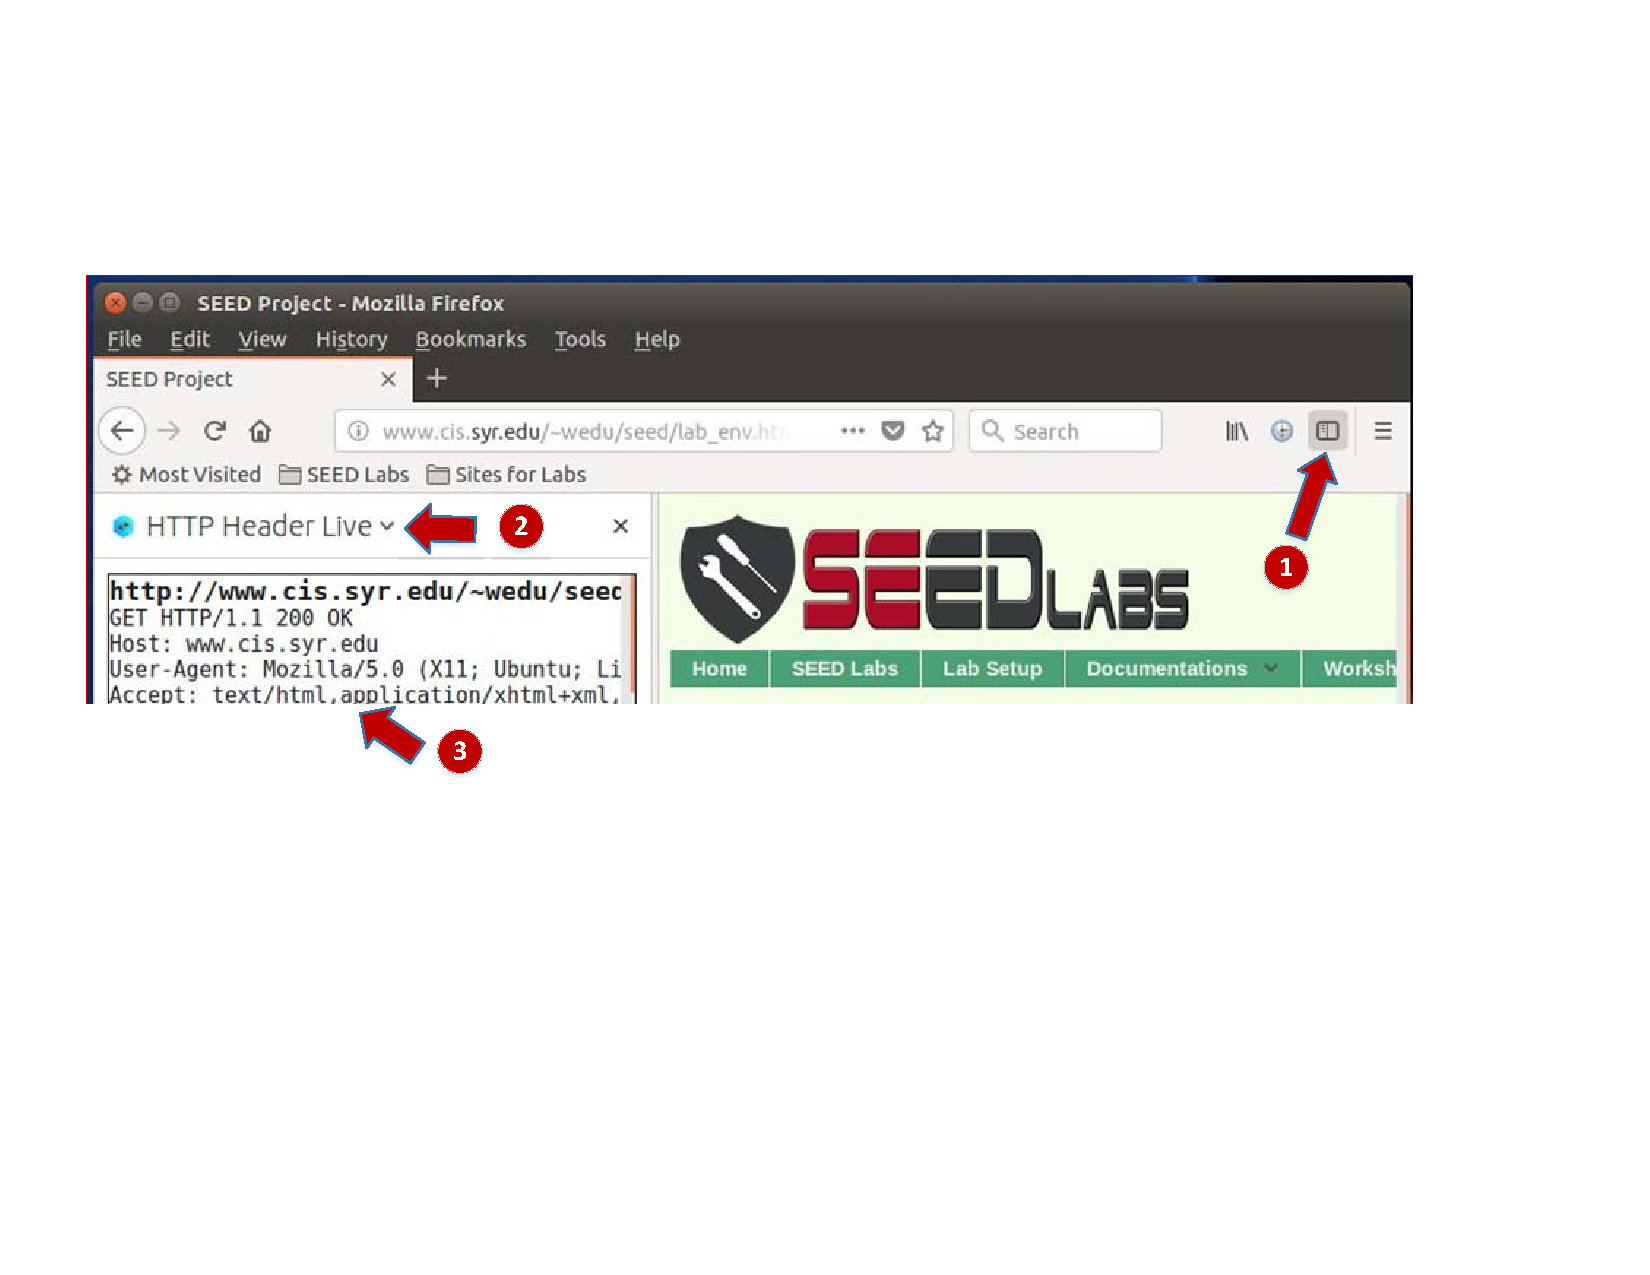
\includegraphics[width=0.85\textwidth]{\devtoolFigs/HTTPHeaderLive.pdf}
\end{center}
\caption{Enable the HTTP Header Live Add-on}
\label{web:fig:httpheader}
\end{figure}




% -------------------------------------------
% SUBSECTION
% ------------------------------------------- 
\subsection{Using the Web Developer Tool to Inspect HTTP Headers}
\label{web:sec:web_dev_tools}


There is
another tool provided by Firefox that can be quite useful 
in inspecting HTTP headers. 
The tool is the Web Developer Network Tool.  In this
section, we cover some of the important features of the tool. 
The Web Developer Network Tool can be enabled via the following navigation: 


\begin{lstlisting}
Click Firefox's top right menu --> Web Developer --> Network
 or 
Click the "Tools" menu --> Web Developer --> Network 
\end{lstlisting}


We use the user login page in Elgg as an example. 
Figure~\ref{fig:webdevtools_01_request} shows the Network Tool showing the HTTP POST request
that was used for login.

\begin{figure}[htb]
\begin{center}
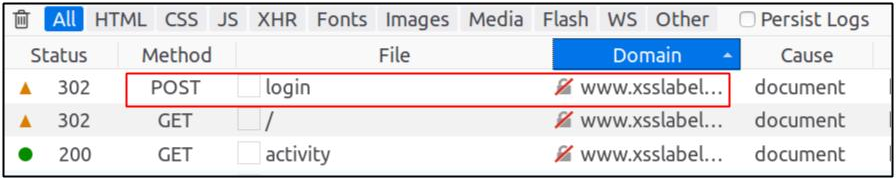
\includegraphics[width=0.8\textwidth]{\devtoolFigs/webdevtools_01_request.png}
\end{center}
\caption{HTTP Request in Web Developer Network Tool}
\label{fig:webdevtools_01_request}
\end{figure}

To further see the details of the request, we can click on a particular HTTP request and the
tool will show the information in two panes (see Figure~\ref{fig:webdevtools_02_two_panes}). 

\begin{figure}[htb]
\begin{center}
	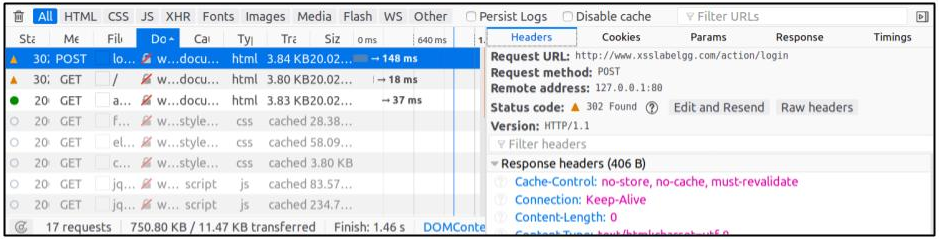
\includegraphics[width=0.95\textwidth]{\devtoolFigs/webdevtools_02_two_panes.png}
\end{center}
\caption{HTTP Request and Request Details in Two Panes}
\label{fig:webdevtools_02_two_panes}
\end{figure}



The details of the selected request will be visible in the right pane.
Figure~\ref{fig:webdevtools_03_post_headers} shows the details of the login request in the
\texttt{Headers} tab (details include URL, request method, and cookie). One can observe both
request and response headers in the right pane. To check the parameters involved in an HTTP
request, we can use the \texttt{Params} tab. Figure~\ref{fig:webdevtools_03_post_params} shows
the parameter sent in the login request to Elgg, including \texttt{username} and
\texttt{password}. The tool can be used to inspect HTTP GET requests in a similar manner to HTTP POST requests.

\begin{figure}[htb]
 \centering
 \subfigure[HTTP Request Headers]{
        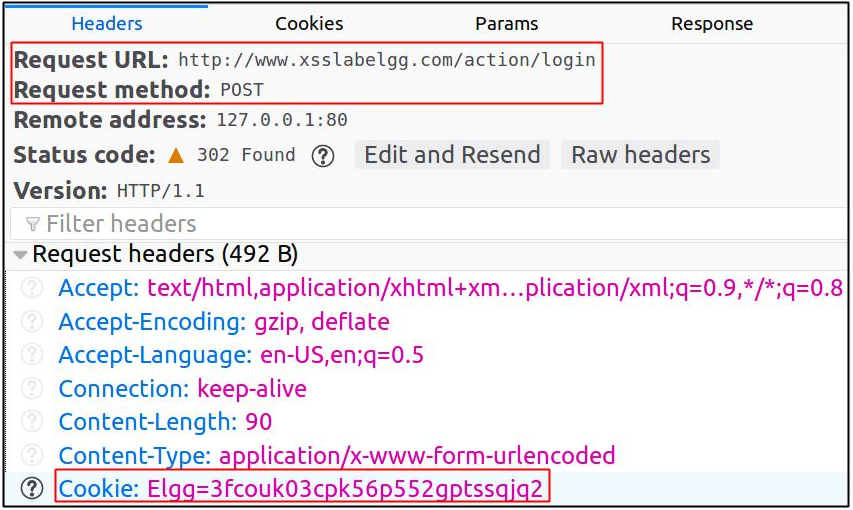
\includegraphics[width=0.6\textwidth]{\devtoolFigs/webdevtools_03-1.png}
        \label{fig:webdevtools_03_post_headers}
 }
 \subfigure[HTTP Request Parameters]{
        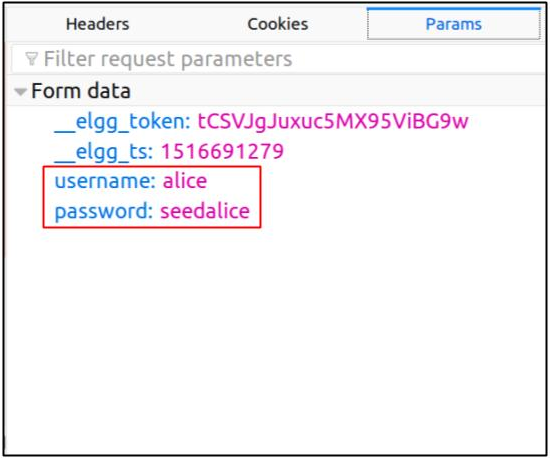
\includegraphics[width=0.35\textwidth]{\devtoolFigs/webdevtools_03-2.png}
        \label{fig:webdevtools_03_post_params}
 }
 \caption{HTTP Headers and Parameters}
\end{figure}


\paragraph{Font Size.} The default font size of Web Developer Tools window is quite small. It
can be increased by focusing click anywhere in the Network Tool window, and then using
\texttt{Ctrl} and \texttt{+} button.


% -------------------------------------------
% SUBSECTION
% -------------------------------------------
\subsection{JavaScript Debugging}
\label{web:sec:jsdebugging}

We may also need to debug our JavaScript code. Firefox's Developer Tool can also help debug
JavaScript code. It can point us to the precise places where errors occur. The following
instruction shows how to enable this debugging tool:

\begin{lstlisting}
 Click the "Tools" menu --> Web Developer --> Web Console
 or use the Shift+Ctrl+K shortcut.
\end{lstlisting}


Once we are in the web console, click the {\tt JS} tab. Click the downward pointing arrowhead
beside {\tt JS} and ensure there is a check mark beside {\tt Error}. If you are also interested
in Warning messages, click {\tt Warning}. See Figure~\ref{devtool:fig:errocheckmark}.


\begin{figure}[htb]
\begin{center}
  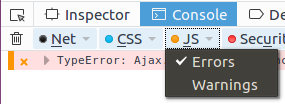
\includegraphics[width=0.4\textwidth]{\devtoolFigs/errorCheckMark.png}
\end{center}
\caption{Debugging JavaScript Code (1)}
\label{devtool:fig:errocheckmark}
\end{figure}
 

If there are any errors in the code, a message will display in the console. The line that
caused the error appears on the right side of the error message in the console. Click on the
line number and you will be taken to the exact place that has the error.
See Figure~\ref{devtool:fig:console}.


\begin{figure}[htb]
\begin{center}
  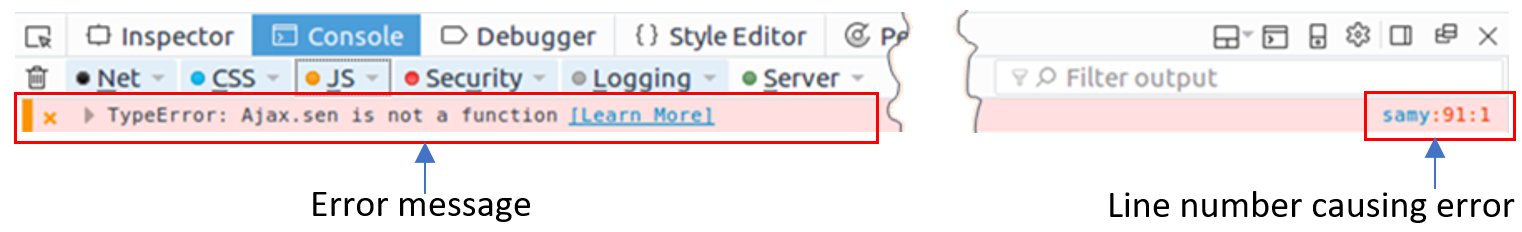
\includegraphics[width=1.0\textwidth]{\devtoolFigs/consoleError2.png}
\end{center}
\caption{Debugging JavaScript Code (2)}
\label{devtool:fig:console}
\end{figure}
 




 

%%%%%%%%%%%%%%%%%%%%%%%%%%%%%%%%%%%%%%%%



% *******************************************
% SECTION
% ******************************************* 
\section{Submission}


%%%%%%%%%%%%%%%%%%%%%%%%%%%%%%%%%%%%%%%%

You need to submit a detailed lab report, with screenshots,
to describe what you have done and what you have observed.
You also need to provide explanation
to the observations that are interesting or surprising.
Please also list the important code snippets followed by
explanation. Simply attaching code without any explanation will not
receive credits.

%%%%%%%%%%%%%%%%%%%%%%%%%%%%%%%%%%%%%%%%



\end{document}



